% -*- root: ../main.tex -*-
\chapter{Design di Dettaglio}
Fin dall'analisi del progetto è stato chiaro che il target dell'applicazione fosse
ampio, infatti l'insieme degli utenti interessati comprende chiunque abbia la
necessità di consultare delle previsioni del meteo.
Per questo motivo, le interfacce e il funzionamento dell'applicazione sono
stati progettati per essere adoperati anche dagli utenti meno esperti.\\

Come tutti i programmi, il progetto è costituito da parte frontend e backend.
Essi denotano rispettivamente la parte visibile all'utente di un programma e con cui egli può interagire —tipicamente un'interfaccia utente— e la parte che permette l'effettivo funzionamento di queste interazioni. Il frontend, nella sua accezione più generale, è responsabile dell'acquisizione dei dati di ingresso e della loro elaborazione con modalità conformi a specifiche predefinite e invarianti, tali da renderli utilizzabili dal backend. Il collegamento del frontend al backend è un caso particolare di interfaccia.
\section{Frontend}
In seguito ad un'analisi preliminare del problema sono stati prodotti dei mockup
della grafica per dare l'idea delle funzionalità e dei requisiti dell'applicativo. Le
pagine effettive si sono evolute durante lo sviluppo ma mantengono le linee guida
dei mockup.

\begin{figure}[H]
    \caption{Home}
    \label{fig:Home}
    \centering
    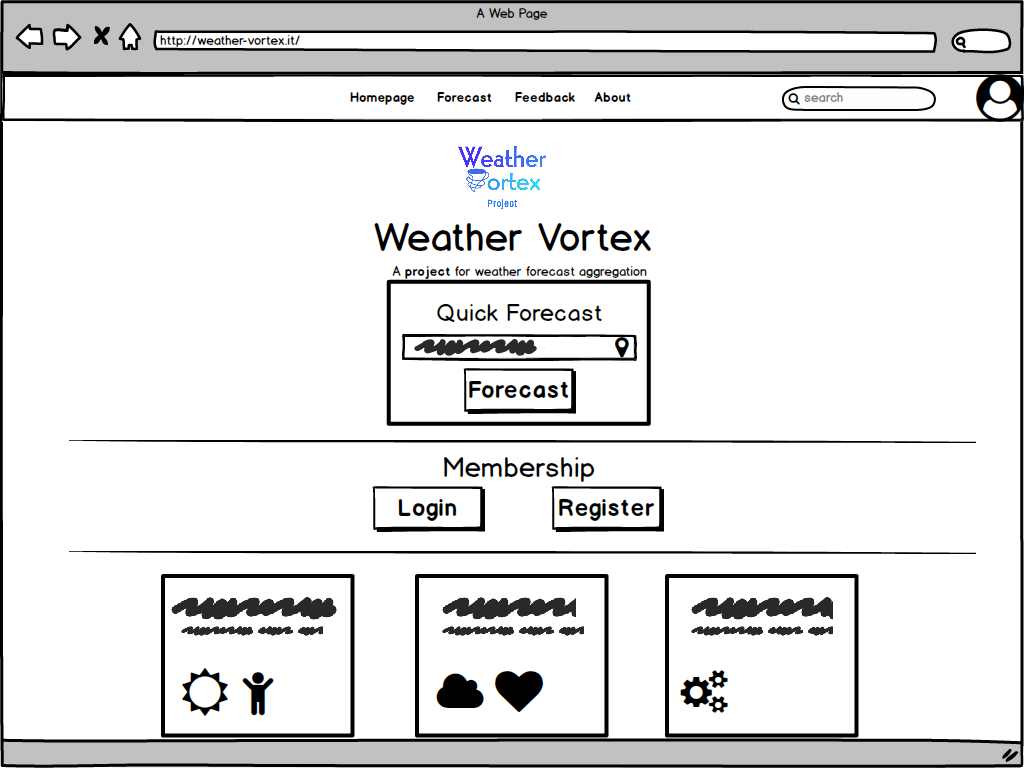
\includegraphics[width=0.5\textwidth]{MockUps/homepage.png}
\end{figure}
La homepage è la pagina principale di presentazione, da cui si può accedere alle previsioni e alle pagine di autenticazione.
\begin{figure}[H]
    \caption{Login}
    \label{fig:Home}
    \centering
    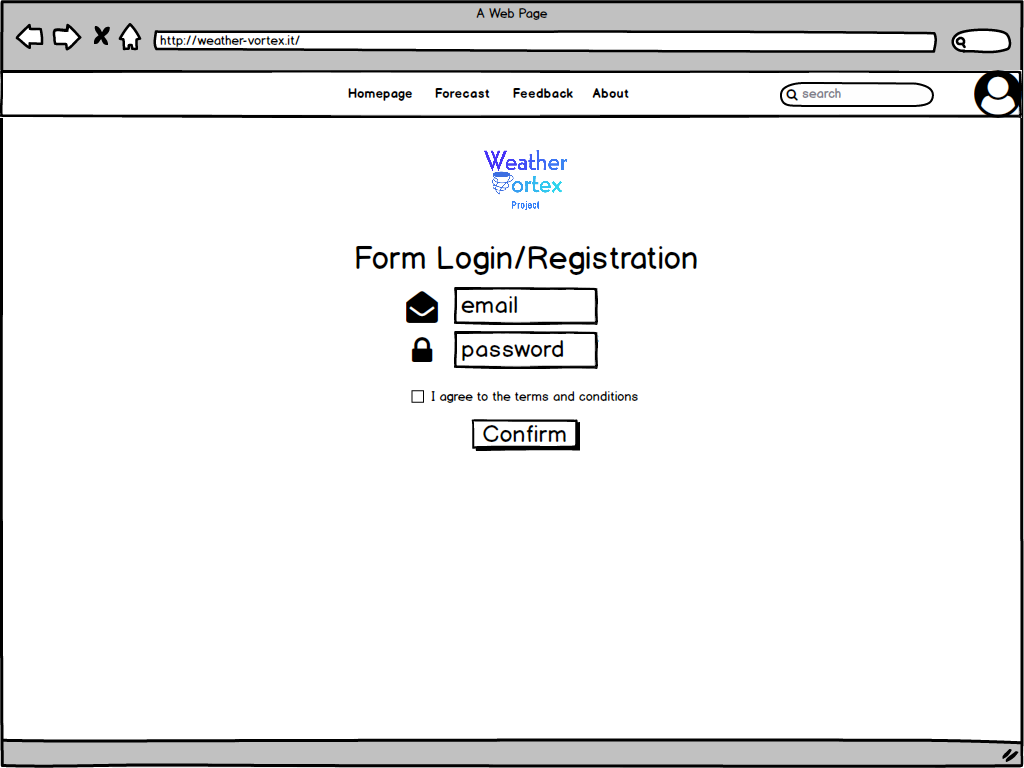
\includegraphics[width=0.5\textwidth]{MockUps/Login_Register.png}
\end{figure}

Viene pensata una pagina di login classica con la possibilità di recuperare la password e una pagina di registrazione. Effettuata la registrazione viene chiesto agli utenti di completare la propria iscrizione, e per questo gli viene inviata una email di conferma.

\begin{figure}[H]
    \caption{Forecast}
    \label{fig:Home}
    \centering
    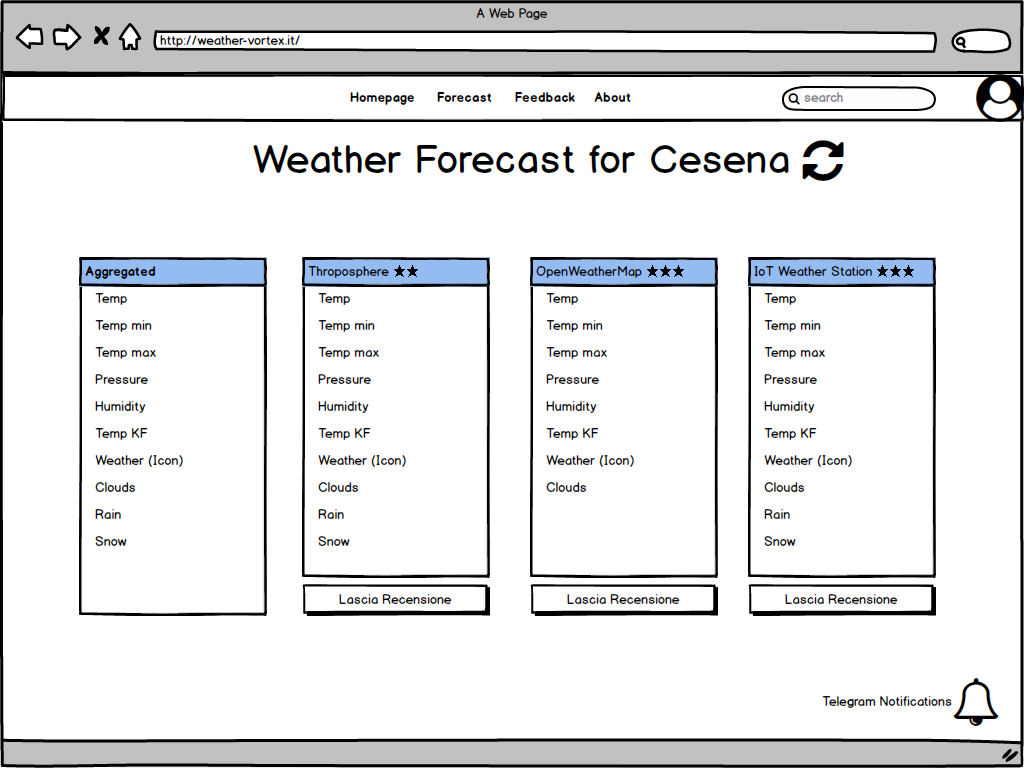
\includegraphics[width=0.5\textwidth]{MockUps/forecast.png}
\end{figure}
Il fulcro dell'applicazione è sicuramente la pagina delle previsioni. Fin da subito si è pensato di raggruppare in schede le previsioni dei vari provider e l'aggregazione. Ogni scheda rappresenta un provider e oltre alla stringa di descrizione del meteo contiene altre informazioni quali la temperatura massima e minima, la pressione, l'umidità, la quantità di nuvole, la quantità di pioggia e la quantità di neve. 
Rispetto al mockup iniziale sono stati aggiunti dei componenti fondamentali alla pagina finale, tra cui una barra di testo per inserire la località e una map-icon per richiedere le coordinate geografiche attuali, con due bottoni a lato per far visualizzare il tempo attuale o quello dei prossimi tre giorni. Nell'opzione previsioni future si ha a disposizione un tooltip di bottoni per precisare il giorno specifico e uno slider per conoscere le varie previsioni orarie.

\begin{figure}[H]
    \caption{Feedbacks}
    \label{fig:Home}
    \centering
    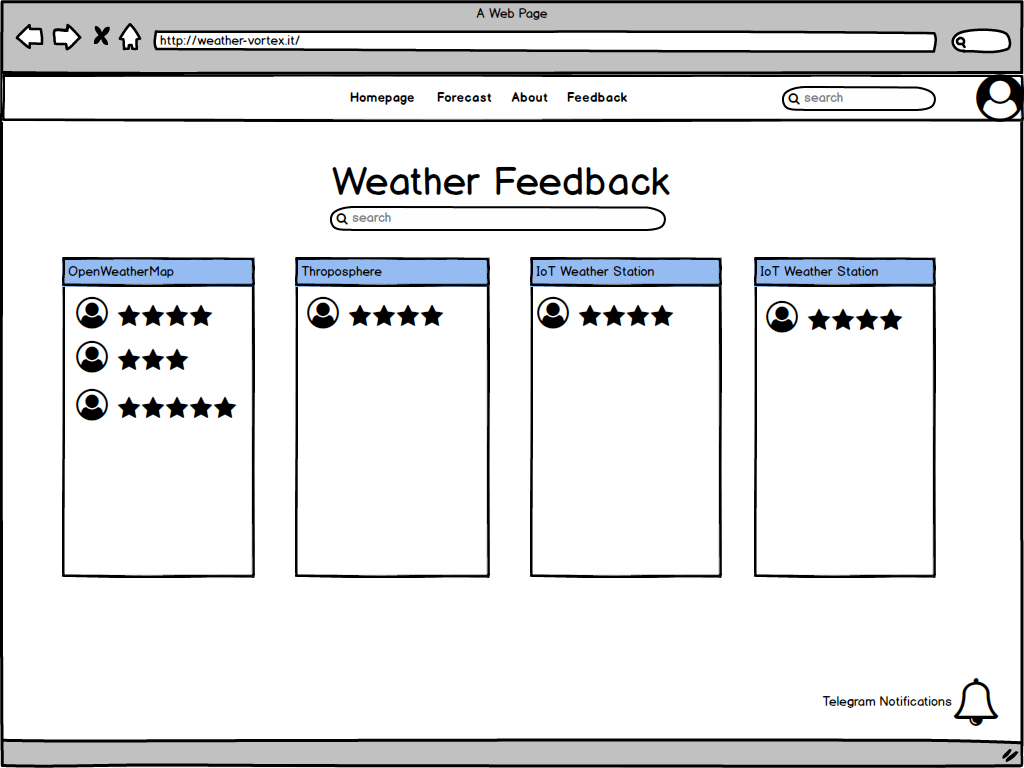
\includegraphics[width=0.5\textwidth]{MockUps/feedback.png}
\end{figure}
Anche nella pagina delle recensioni è presente uno slider di schede, una per ogni provider. 
Ogni provider contiene diversi campi, ognuno rappresenta una recensione che è stata rilasciata. Ogni campo è cliccabile per permettere di visualizzare il profilo pubblico dell'utente che ha rilasciato la recensione. All'estremità di ogni scheda, se si è autenticati, sarà presente il bottone per aggiungere una nuova recensione.
In cima ad ogni card si è deciso di far visualizzare una statistica, calcolata come media dei rating di quel provider. Si tratta di un indice di affidabilità che calcola l'accuratezza della previsione, basandosi sull'opinione delle altre persone.



\begin{figure}[H]
    \caption{Aggiunta di una recensione}
    \label{fig:Home}
    \centering
    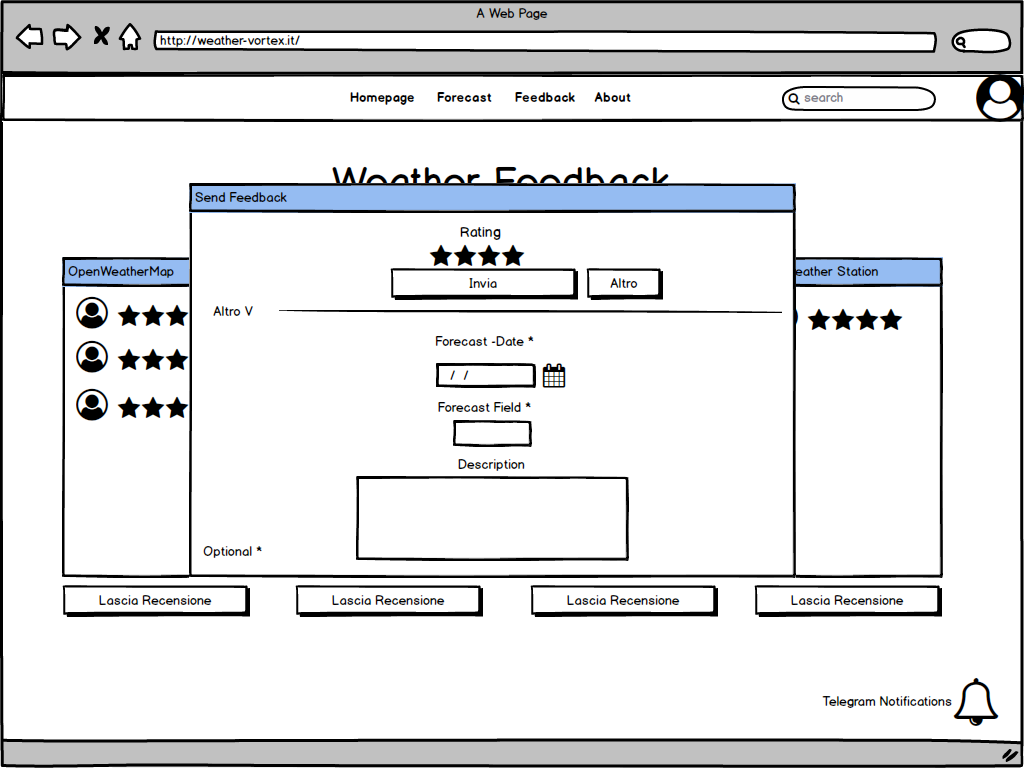
\includegraphics[width=0.5\textwidth]{MockUps/sendFeedback.png}
\end{figure}

\begin{figure}[H]
    \caption{Profilo privato}
    \label{fig:Home}
    \centering
    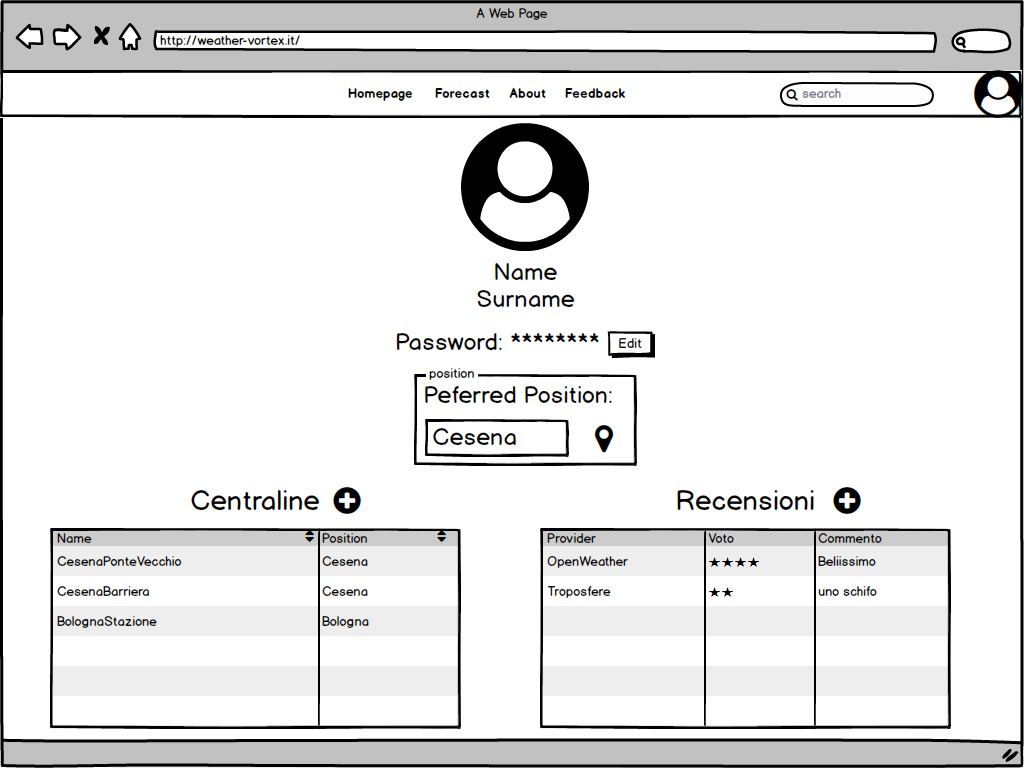
\includegraphics[width=0.5\textwidth]{MockUps/Private Profile.png}
\end{figure}
La pagina del profilo privato dà la possibilità ad ogni utente di gestire le proprie informazioni. Contiene inoltre una card con la possibilità di modificare la propria password e la propria posizione preferita. 
Inoltre per visualizzare le proprie centraline e le proprie recensioni si sono usate due tabelle, che permettono anche di fare operazioni di aggiunta, modifica e cancellazione.\\

Sulla falsa riga del Profilo Privato è stata anche realizzata la pagina del Profilo Pubblico.

\begin{figure}[H]
    \caption{About}
    \label{fig:Home}
    \centering
    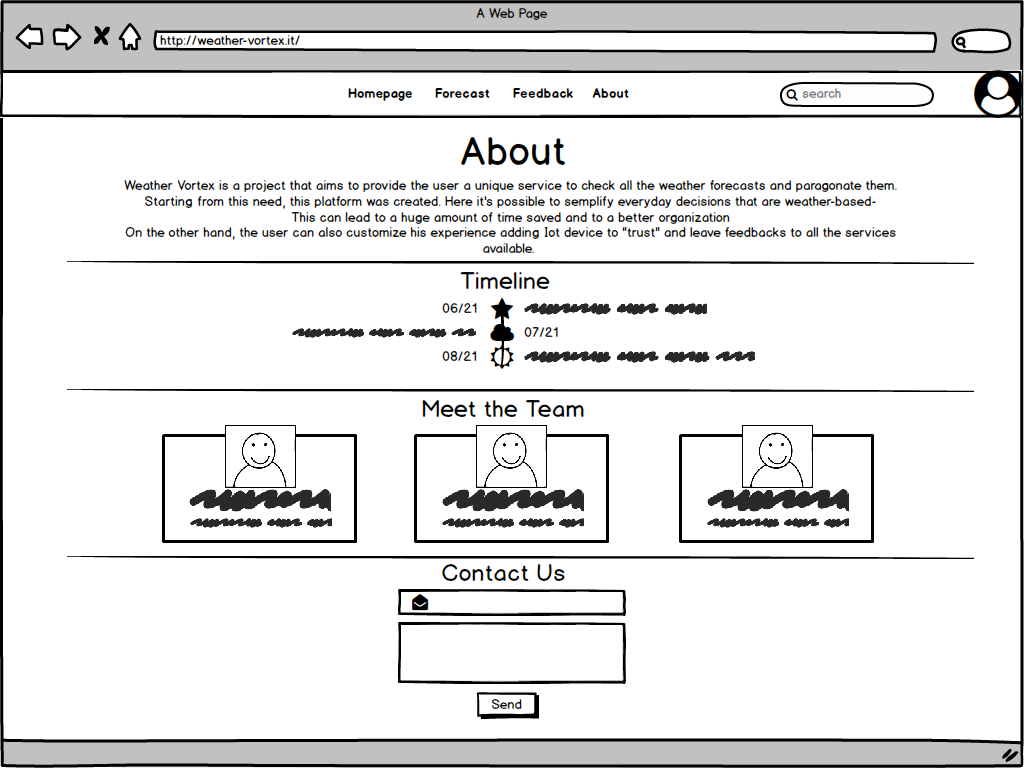
\includegraphics[width=0.5\textwidth]{MockUps/about.png}
\end{figure}
Infine una pagina per i contatti che consente l'inserimento di un messaggio/ticket
per il supporto tecnico e alcune informazioni sul team di sviluppo.

\subsection{Notifiche}
A inizio progetto si era preventivato un sistema di notifiche sia push che via email e telegram. 
Alla fine è stato implementato solo un sistema di notifiche via email, che invia all'utente notizie sul tempo attuale della propria posizione preferita. 



\section{Backend}
Viene ora mostrato il database utilizzato dall'applicazione:

FIGURA DATABASE
\subsection{Collezioni}
Ci sono ha cinque collezioni che sono il fulcro dell'applicazione, essi si trovano nella cartella models. Essi costituiscono un modello di dati da salvare in MongoDB, che vengono usati per istanziare oggetti che saranno automaticamente dotati di metodi per svolgere le classiche operazioni CRUD.
\begin{itemize}
\item user - Rappresenta il modello dell'utente. I suoi campi sono:
\begin{itemize}
\item
\end{itemize}
\item feedback - Rappresenta il modello della recensione. I suoi campi sono: 
\item location - Rappresenta il modello della località. I suoi campi sono:
con un nome e le coordinate geografiche espresse in latitudine e longitudine.
\item provider - Rappresenta il modello del provider che fornisce il meteo, contiene una lista di recensioni e un indice di affidabilità.
\item station - Rappresenta  il modello della centralina.
\end{itemize}
\subsection{Risorse}
Il backend è stato strutturato secondo le seguenti risorse, che si trovano nella cartella storage:
\begin{itemize}
\item auth - risorsa che manipola il modello user e serve per registrare, autenticare gli utenti, cancellarli, recuperarne le
informazioni o aggiornarle. 
\item feedback - risorsa per gestire le recensioni degli utenti sui vari provider meteo.
\item location - risorsa per cercare di recuperare le informazioni di localizzazione di una determinata località.
\item station - risorsa per gestire le varie centraline.
\item openweathermap - risorsa per gestire le richieste dall'api openweathermap e recuperare le previsioni meteo desiderate.
\item troposphere - risorsa per gestire le richieste dall'api troposphere e recuperare le previsioni meteo desiderate.
\item users - risorsa per recuperare un determinato utente e recuperarne i feedbacks e le stazioni.

\end{itemize}





